\section{Tests}

\subsection{Type of tests}

\subsubsection{JUnit}

\begin{figure}[h]
	\centering
	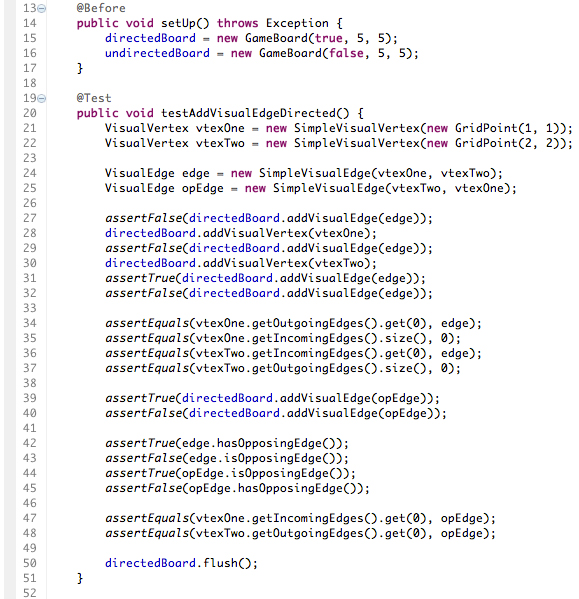
\includegraphics[width=.95\textwidth]{junit_screenshot.jpg}
	\caption{JUnit test for the GameBoard.}
	\label{img:screenJUnit}
\end{figure}
\emph{JUnit} is the most commonly used framework to write repeatable unit tests for Java applications.\par
Every object can be tested separately using defined input values and expected output values. Methods and object correlations not working as intended will attract attention reliably.\par

\subsubsection{Sikuli}

\begin{figure}[!h]
	\centering
	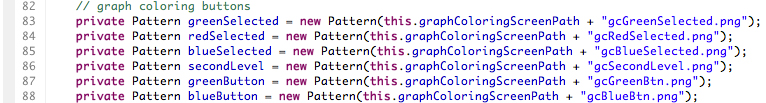
\includegraphics[width=.95\textwidth]{sikuli_screenshot_1.jpg}
	\caption{GUI elements defined for tests with Sikuli.}
	\label{img:screenSikuli1}
\end{figure}
\begin{figure}[!h]
	\centering
	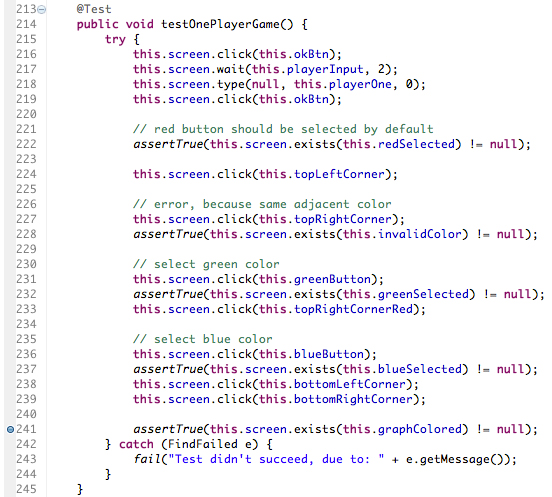
\includegraphics[width=.95\textwidth]{sikuli_screenshot_2.jpg}
	\caption{Sikuli test for the Graph-Coloring single-player game.}
	\label{img:screenSikuli2}
\end{figure}
For extensive tests of our graphical user interfaces (GUIs), we drew on open-source \emph{Project SIKULI}. Sikuli is a visual technology to automate and test those interfaces using screenshots.\par
The tests are developed using a pseudo language connected with cropped images from the application's screenshots. A click on a button for instance would look like this:\par
\begin{figure}[!h]
	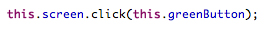
\includegraphics{sikuli_screenshot_3.jpg}
	\label{img:screenSikuli3}
\end{figure}
Every possible item can be clicked on, no matter if its a real button, text field etc. Sikuli simply looks for the provided screenshot in the GUI and simulates a mouse click on the item that it found. In pseudo code the test developer then defines click paths and assertions. Those assertions again are cropped images from screenshots. If they appear somewhere after the click, the test passes. Otherwise it fails.\par
Once all clickable items are saved as screenshot parts, every possible scenario can be executed semi-automatically. These tests can also be designed as regression test.\par

\subsubsection{Manual tests}

As defined in the \emph{Pflichtenheft}, we conducted 18 test cases and four test scenarios. As those have been defined before design and implementation, they give some indication of whether the framework and the games in general have been deployed as planned.\par

\subsection{Implementation details}
We implemented unit tests during the implementation phase, achieving a code coverage in some packages of almost 90\%\todo{Verify number}.\par
A lot more unit test have been added since and by the end of the validation phase, we beat the number of 98\% of code coverage with unit tests.\par
However, a lot of possible errors could be embedded in the GUIs. And as Java does not provide easy and free frameworks for GUI testing, we used the above described Sikuli to act out almost all possible click combinations in both \gameexplorer and \emph{GameWindow}.\par
The - mainly positive - results of all tests are outlined in the next sections.\par